%!TeX program = xelatex
\documentclass{SYSUReport}

\usepackage{amsmath}
\usepackage{array}
\usepackage{booktabs}
\usepackage{graphicx}
\usepackage{listings}
\usepackage{xcolor}
\setlength{\headheight}{15pt}

\definecolor{codegray}{RGB}{75,85,99}
\definecolor{codeblue}{RGB}{30,64,175}
\definecolor{codegreen}{RGB}{22,101,52}
\definecolor{codepurple}{RGB}{126,34,206}

\lstdefinestyle{mystyle}{
    backgroundcolor=\color{gray!8},
    basicstyle=\ttfamily\small,
    keywordstyle=\color{codeblue},
    commentstyle=\color{codegreen},
    stringstyle=\color{codepurple},
    numbers=left,
    numberstyle=\tiny\color{codegray},
    frame=single,
    rulecolor=\color{gray!45},
    breaklines=true,
    keepspaces=true,
    showstringspaces=false,
    columns=fullflexible,
    captionpos=b
}
\lstset{style=mystyle}

\headl{学号 24341025}
\headc{}
\headr{数据安全和隐私保护}
\lessonTitle{数据安全和隐私保护}
\reportTitle{实验一 实验基础工具使用}
\stuname{黄志鹏}
\stuid{24341025}
\inst{网络空间安全学院}
\major{网络空间安全}
\date{2026 年 9 月 13 日}

\begin{document}

\cover
\thispagestyle{empty}
\clearpage

\tableofcontents
\clearpage

\pagenumbering{arabic}
\setcounter{page}{1}

\section{实验要求}

本次实验围绕科研代码管理、AI 辅助编程和实验报告撰写三个基础环节展开。具体要求如下：

\begin{enumerate}
    \item 掌握 LaTeX 中插入图片的基本方法，至少插入一张实验结果图，为图片设置规范的图题和标签，并在正文中使用交叉引用；
    \item 掌握 Git 和 GitHub 的仓库创建、克隆、提交、上传和更新流程，提交前使用 \texttt{git status}、\texttt{git diff} 和 \texttt{git log} 核对变更；
    \item 完成 Codex 的基本使用，了解 CC Switch 的供应商配置与切换方法，并使用 Codex 完成至少一次代码阅读、生成或修改任务；
    \item 报告应记录关键命令、重要操作、运行结果、代码修改情况和实验总结，且不得泄露 API Key、密码或访问令牌。
\end{enumerate}

本报告以一个仅依赖 Python 标准库的文本词频统计程序作为 Codex 辅助编程任务，并用程序输出制作 LaTeX 矢量图。本次作业的 GitHub 仓库为 \url{https://github.com/HUANGZHP/coursework_in_sysu}，\texttt{main} 分支已完成推送；本地 bare remote 用于补充验证 push/pull 流程。

\section{实验原理}

\subsection{Git 版本控制原理}

Git 将一次修改依次保存在工作区、暂存区和本地仓库中。工作区用于编辑文件，\texttt{git add} 将明确选择的变化放入暂存区，\texttt{git commit} 把暂存内容记录为一个带有说明的版本。\texttt{git status} 显示整体状态，\texttt{git diff} 检查未暂存修改，\texttt{git diff --staged} 检查即将提交的修改，\texttt{git log} 用于追踪历史。远程同步时，\texttt{git push} 将本地提交发送到远程仓库，\texttt{git pull} 获取远程提交并合并到本地。

\subsection{Codex 辅助编程原理}

AI 辅助编程的可靠流程不是直接接受生成结果，而是先让工具读取项目并说明入口，再提出小而明确的任务，审阅准备执行的命令和差异，运行程序与测试，最后使用 Git 独立检查。这样可以把“理解、修改、验证、保存”分成可核对的步骤，降低误改文件、引入依赖或泄露敏感信息的风险。

\subsection{LaTeX 图片排版原理}

LaTeX 通过 \texttt{graphicx} 宏包将图片排入文档，\texttt{caption} 产生图题，\texttt{label} 与 \texttt{ref} 建立交叉引用。对折线图、柱状图和结构图等结果，优先使用 PDF 或 SVG 等矢量格式，可以在改变版面尺寸时保持文字和曲线清晰。本实验使用 PDF 矢量柱状图记录词频结果。

\section{实验设置}

\begin{table}[htbp]
    \centering
    \caption{实验环境}
    \label{tab:environment}
    \begin{tabular}{>{\raggedright\arraybackslash}p{0.28\textwidth}p{0.58\textwidth}}
        \toprule
        项目 & 设置 \\
        \midrule
        操作系统与终端 & Windows，PowerShell \\
        Git & git version 2.53.0.windows.3 \\
        Python & Python 3.12.14 \\
        LaTeX & MiKTeX-XeTeX 4.15，MiKTeX 25.4 \\
        Codex & codex-cli 0.153.4；使用 Codex 桌面会话辅助完成任务 \\
        CC Switch & 检测到 Windows 客户端可执行文件；切换时不在代码或报告中保存密钥 \\
        \bottomrule
    \end{tabular}
\end{table}

程序入口为 \texttt{code/text\_stats.py}，输入文件为 \texttt{code/sample.txt}。程序使用正则表达式提取英文单词、数字和中文字符；英文单词统一转换为小写，中文按单字统计，因此无需安装第三方分词包。实验命令为：

\begin{lstlisting}[language=bash,caption={实验复现命令}]
python code/text_stats.py code/sample.txt --top 8
python -m py_compile code/text_stats.py
\end{lstlisting}

本地 Git 提交使用仓库级示例身份 \texttt{实验报告作者 <student@example.com>}，仅用于演示提交记录，不代表 GitHub 登录凭据。实验过程中没有在环境变量、配置文件、代码、报告或图片中写入 API Key。

\section{实验过程}

\subsection{LaTeX 图片排版}

首先将实验图片统一放入 \texttt{result} 目录，并使用短英文文件名。程序运行后得到 67 个 token 和 56 个不同 token，取出现次数最高的 8 项制作柱状图。图~\ref{fig:frequency} 使用 PDF 格式，正文通过标签引用该图，放大后仍可保持柱线和文字的清晰度。

\begin{figure}[htbp]
    \centering
    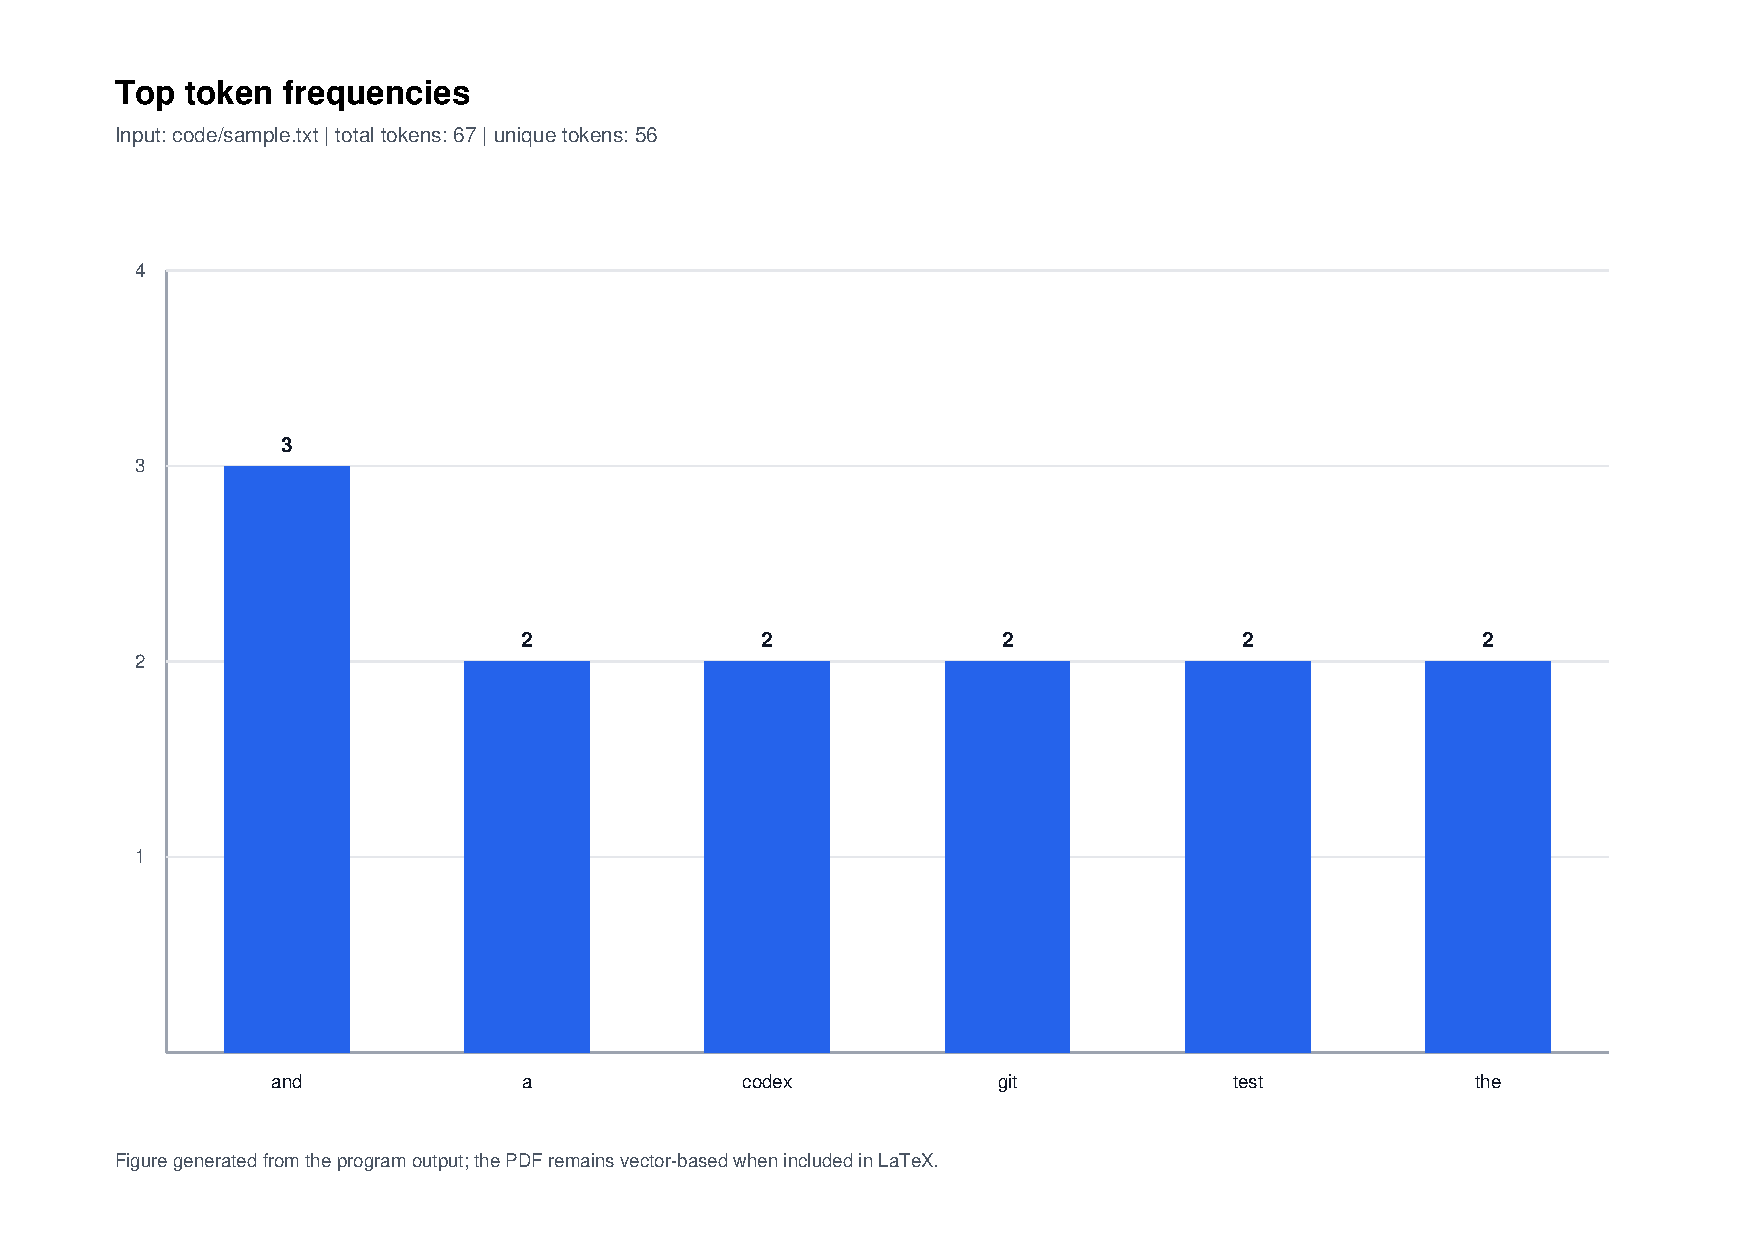
\includegraphics[width=0.86\textwidth]{result/text_stats_bar.pdf}
    \caption{文本词频统计结果}
    \label{fig:frequency}
\end{figure}

\subsection{Git 仓库与提交}

项目初始目录不是 Git 仓库，因此先在项目根目录执行初始化并设置仓库级提交身份：

\begin{lstlisting}[language=bash,caption={初始化仓库与第一次提交}]
git init -b main
git config user.name "实验报告作者"
git config user.email "student@example.com"
git add README.md .gitignore code/text_stats.py code/sample.txt result/README.md report/README.md
git diff --staged
git commit -m "add first experiment program"
\end{lstlisting}

第一次提交只包含 README、程序和输入样例。完成程序测试、结果图和报告后，先检查状态与差异，再完成第二次提交：

\begin{lstlisting}[language=bash,caption={检查修改并提交实验结果}]
git status
git diff
git add main.tex result/text_stats_output.txt result/text_stats_bar.pdf
git diff --staged
git commit -m "add experiment result and report"
\end{lstlisting}

为了验证远程同步语义，本地先在仓库的 Git 元数据目录中建立了一个 bare remote，执行了与 GitHub 相同的命令：

\begin{lstlisting}[language=bash,caption={远程推送与更新同步}]
git remote add origin .git/remote.git
git push -u origin main
# 在另一个克隆目录修改 README 并提交、推送
git pull --ff-only
git log --oneline --graph --decorate -n 5
\end{lstlisting}

完成本地验证后，本次又将同一 \texttt{main} 分支推送到上述个人 GitHub 仓库，远程名为 \texttt{github}，远程分支与本地提交 \texttt{d6db243} 一致。认证通过 SSH 密钥完成，私钥没有写入命令、脚本或报告。本地最终提交历史记录见图~\ref{fig:gitrecord} 和附录输出文件。

\begin{figure}[htbp]
    \centering
    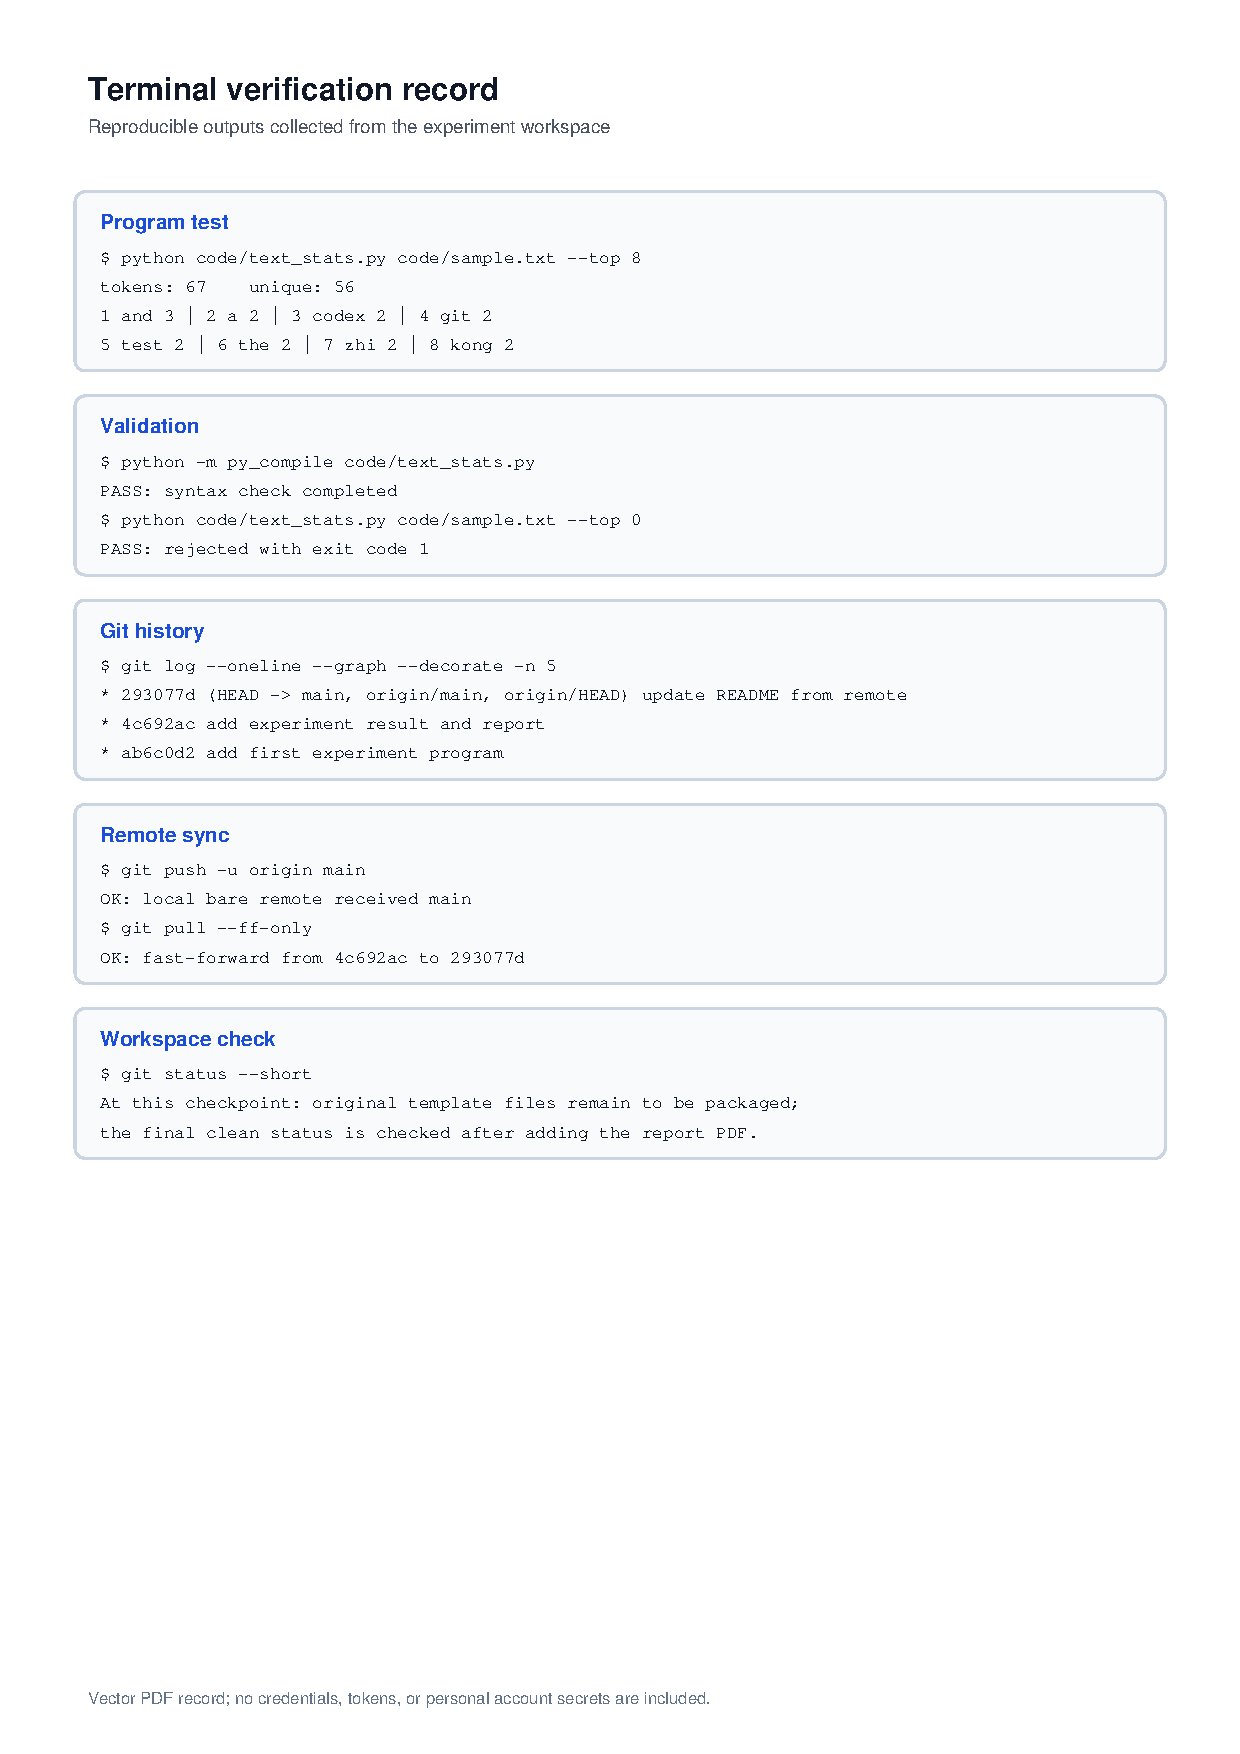
\includegraphics[width=0.94\textwidth]{result/terminal_verification.pdf}
    \caption{关键命令执行记录}
    \label{fig:gitrecord}
\end{figure}

\subsection{Codex 与 CC Switch}

本次任务中先让 Codex 阅读项目，确认项目只有 LaTeX 模板和实验说明，没有现成代码入口；随后提出“生成一个仅使用标准库、支持 UTF-8、可指定输出条数的文本词频统计程序，并给出测试命令”的小任务。生成后逐行检查了正则表达式、输入文件编码、排序规则和非法参数处理，再独立运行程序、语法检查和 \texttt{--top 0} 边界测试，最后用 Git 检查文件变化。

本机已检测到 Codex CLI 和 CC Switch Windows 客户端。CC Switch 的安全使用步骤是：打开 Codex 页面，添加供应商，按供应商文档填写名称、Endpoint URL 和模型，保存后启用供应商，重新打开 Codex，再用 \texttt{/status} 和一个小问题检查生效情况。API Key 只应保存在受保护的本地配置或系统凭据中，不应出现在报告、截图、Git 仓库或命令历史中。本报告只记录配置流程和字段名称，不记录任何认证值。

\subsection{代码修改情况}

新增的程序入口如下。程序对不存在的输入文件和非正整数 \texttt{--top} 参数主动报错，避免生成误导性的空结果。

\lstinputlisting[language=Python,caption={文本词频统计程序}]{code/text_stats.py}

\section{实验结果与分析}

正常运行输出如下，结果文件保存在 \texttt{result/text\_stats\_output.txt}：

\lstinputlisting[caption={程序运行输出}]{result/text_stats_output.txt}

实验结果表明，样例共提取 67 个 token，其中不同 token 为 56 个；出现次数最多的是 \texttt{and}，共 3 次。\texttt{a}、\texttt{codex}、\texttt{git}、\texttt{test} 和 \texttt{the} 各出现 2 次。中英文混合输入能够被统一处理，英文大小写不会造成重复计数，中文字符则按字符进行可复现的简单统计。

边界测试中，执行 \verb|python code/text_stats.py code/sample.txt --top 0| 得到错误信息“--top must be a positive integer”，进程以非零状态退出，说明命令行参数校验生效。\verb|python -m py_compile code/text_stats.py| 也顺利完成，说明程序不存在语法错误。

\section{实验总结}

通过本次实验，我把一个小程序从需求、实现、运行、结果保存到版本提交完整地走了一遍。Git 的价值不仅是备份，更重要的是在提交前通过 \texttt{status} 和 \texttt{diff} 明确“改了什么”，在提交后通过 \texttt{log} 追溯“什么时候改的”。因此一次提交应只包含一个清晰目标，暂存时也应明确列出文件。

使用 Codex 时，先限定任务范围再审阅修改内容十分重要。生成代码不能替代运行测试，能运行也不能替代检查依赖、输入边界和敏感信息。CC Switch 提供了供应商切换便利，但本地代理和多供应商配置会增加新的信任边界，密钥保护、端口暴露和配置恢复都需要单独检查。

最后，LaTeX 报告中的图片不应只是“贴上去”。将结果导出为 PDF 矢量图、设置图题和标签，并在正文中引用，能够让实验结论和证据建立清晰对应关系。后续实验中我会继续保持“先复现、再分析、后提交”的工作习惯。

\appendix
\section{最终 Git 历史}

下面的记录由最终本地仓库直接生成，保留了第一次程序提交、第二次报告提交以及远程 README 更新后的同步结果。

\lstinputlisting[caption={最终 Git 提交历史}]{result/git_log.txt}

\section{最终工作区状态}

\lstinputlisting[caption={最终 Git 状态}]{result/git_status.txt}

\end{document}
